\documentclass[10pt,twocolumn,letterpaper]{article}

\usepackage{cvpr}
\usepackage{times}
\usepackage{epsfig}
\usepackage{graphicx}
\usepackage{amsmath}
\usepackage{amssymb}
\usepackage{booktabs}
\usepackage{tabularx}
\usepackage{array}
\usepackage[breaklinks=true,bookmarks=false]{hyperref}

\cvprfinalcopy
\def\cvprPaperID{0000}
\def\httilde{\mbox{\tt\raisebox{-.5ex}{\symbol{126}}}}
\setcounter{page}{1}

\newcommand{\ours}{V4-LF}
\newcommand{\srgb}{S_{\mathrm{rgb}}}
\newcommand{\sdelta}{S_{\Delta}}
\newcommand{\lrxn}{\mathcal{L}_{\mathrm{rxn}}}
\newcommand{\lossdiff}{\mathcal{L}_{\mathrm{diff}}}
\newcommand{\losslf}{\mathcal{L}_{\mathrm{lf}}}
\newcommand{\losshf}{\mathcal{L}_{\mathrm{hf}}}
\newcommand{\lossaux}{\mathcal{L}_{\mathrm{aux}}}
\newcommand{\lossreg}{\mathcal{L}_{\mathrm{reg}}}

\begin{document}

\title{From Action-Blind Prediction to Action-Sensitive Driving Video Generation}

\author{Maleeka [Last Name]\\
Stanford University\\
{\tt\small edit-author-info@stanford.edu}
\and
[Project Partner]\\
Stanford University\\
{\tt\small edit-author-info@stanford.edu}}

\maketitle

\begin{abstract}
Pretrained video diffusion transformers can produce plausible driving videos from visual context alone, but this does not make them controllable world models. We study front-camera Waymo future generation: given 49 observed frames at 24 FPS, synthesize the next 72 frames while conditioning on future ego-action signals. The central failure mode is that naive action conditioning either gets ignored or damages the visual prior, producing blur, wobble, or motion collapse. We present a low-frequency action-conditioning objective for a frozen pretrained diffusion transformer with trainable LoRA and action modules. The final model uses full 112D per-frame ego actions, a temporal action bottleneck, low-frequency future-token target and delta losses, and a high-frequency teacher preservation term. On 1,904 validation windows, the no-action visual baseline has exactly zero action sensitivity, while our selected action model reaches $\srgb=2.262$ under counterfactual action perturbations. It preserves near-baseline visual quality: PSNR 17.180 vs. 17.153, SSIM 0.70816 vs. 0.70789, and FVD-style distance 11.747 vs. 11.702. On high-action clips, correct actions outperform zero, shuffled, and reversed-future actions with $\Delta$PSNR $=+0.0019$ and $\Delta$SSIM $=+0.00027$. The effect is modest, but it is the first full-validation evidence in our project that the model is not merely action-sensitive, but slightly action-aligned where future actions matter.
\end{abstract}

\section{Introduction}

Autonomous-driving video prediction is often evaluated as visual future continuation: given past camera frames, predict plausible future frames. This is useful, but it is not sufficient for a driving world model. A world model should answer counterfactual questions: if the same observed scene is followed by a different ego-action sequence, should the generated future change accordingly?

This distinction matters because front-camera driving scenes are strongly constrained by visual context. A model with no access to actions can still produce plausible futures and obtain competitive PSNR, SSIM, or FVD-style scores. But it is action-blind by construction:
\begin{equation}
G(x_{\mathrm{ctx}}, a_{\mathrm{correct}})
=
G(x_{\mathrm{ctx}}, a_{\mathrm{zero}})
=
G(x_{\mathrm{ctx}}, a_{\mathrm{shuffled}}).
\end{equation}
Such a model can be a good conditional video prior, but it is not controllable.

We adapt a pretrained video diffusion transformer into an action-conditioned front-camera future generator. The input is 49 context frames at 24 FPS; the target is the next 72 frames. We condition on future ego-action sequences aligned to the same 121-frame window. The final action representation is a dense 112D vector per frame.

Our main empirical observation is negative before it is positive: simple ways of injecting actions into a pretrained video diffusion transformer fail. Global action tokens, temporal action tokens, and AdaLN-style modulation can make the model react to actions, but they often corrupt the visual pathway. Some variants even improve PSNR and SSIM by smoothing motion and removing high-frequency detail, which makes pixel metrics look better while the video becomes less useful.

The final method, \ours, is built around one hypothesis:
\begin{quote}
\emph{Ego-actions are primarily low-frequency temporal control signals. They should influence coarse future evolution without directly rewriting high-frequency appearance.}
\end{quote}
We implement this with a temporal action bottleneck, low-frequency target and temporal-delta supervision, high-frequency teacher preservation from a corrected no-action visual model, and small residual/gate penalties. The base transformer, text encoder, and VAE are frozen; only LoRA adapters and action-conditioning modules are trained.

Our contribution is not a claim that the final model solves action-conditioned driving video generation. It does not. Instead, the contribution is a controlled empirical finding: action conditioning becomes measurable and slightly semantically aligned when routed through low-frequency temporal structure, while visual quality remains near the no-action baseline.

\section{Related Work}

\textbf{Video diffusion transformers.}
Diffusion models~\cite{ho2020ddpm} and latent diffusion~\cite{rombach2022ldm} provide strong generative priors. Diffusion transformers (DiTs)~\cite{peebles2023dit} replace convolutional UNets with scalable token-based architectures, and recent video models extend this design to long spatiotemporal generation~\cite{brooks2024sora,yang2024cogvideox,kong2024hunyuanvideo,ha2024ltx}. Our work does not train a video generator from scratch. We study whether a pretrained video diffusion transformer can be lightly adapted into an action-conditioned driving predictor using LoRA~\cite{hu2021lora} and external action modules.

\textbf{Controllable video generation.}
Prior work injects controls through adapters, ControlNet-like branches~\cite{zhang2023controlnet}, dense conditioning streams such as VideoComposer~\cite{wang2023videocomposer}, trajectory or camera controls~\cite{wang2024motionctrl}, and in-context conditioning. FullDiT2~\cite{he2025fulldit2}, one of the papers that informed our design, argues that concatenating many condition tokens into a full-attention video DiT is powerful but computationally redundant. This matches our experience: broad action-token exposure can be expressive, but it also risks interfering with visual synthesis. We therefore move away from unrestricted global action tokens toward a bottlenecked latent-time residual.

\textbf{Auxiliary objectives and preservation losses.}
Recent video-diffusion training papers show that auxiliary objectives can improve generation when they are aligned with the structure of the problem. Align4Gen~\cite{lee2025align4gen} aligns intermediate video diffusion features with pretrained vision encoders and emphasizes complementary frequency information. Conditional generative video compression~\cite{yi2025conditionalcompression} uses multi-granular conditioning, role-aware embeddings, and robustness to missing conditions. Enhance-A-Video~\cite{luo2025enhanceavideo} studies temporal attention and the tension between temporal consistency and spatial detail. These works motivated our separation of low-frequency control from high-frequency appearance preservation.

\textbf{Driving world models.}
Generative driving simulators such as GAIA-1~\cite{hu2023gaia1} and DriveDreamer~\cite{wang2023drivedreamer} study controllable video generation for autonomous driving. Our scope is narrower: we do not build a complete simulator. We isolate one adaptation question: can a pretrained diffusion transformer become action-sensitive and action-aligned on Waymo-style front-camera continuation with limited trainable parameters?

\section{Data and Task}

We use Waymo front-camera windows derived from 24 FPS interpolated clips. Each training example is
\begin{equation}
x_{0:120} = (x_0,\ldots,x_{120}),\qquad a_{0:120}\in\mathbb{R}^{121\times112}.
\end{equation}
The model observes frames $x_{0:48}$ and predicts $x_{49:120}$. The loss is applied to the future segment. The action tensor is aligned frame-by-frame to the same 121-frame window. We use 7,992 training windows per epoch and 1,904 validation windows.

\begin{table}[t]
\centering
\caption{Final task setup. All final results use the corrected 24 FPS action-aligned windows and seed 231.}
\small
\begin{tabularx}{\linewidth}{lX}
\toprule
Backbone & Pretrained 2B-parameter video diffusion transformer \\
Input & 49 context frames, front camera, 24 FPS \\
Target & 72 future frames, front camera, 24 FPS \\
Action & 112D per-frame ego-action vector \\
Train windows & 7,992 per epoch \\
Validation windows & 1,904 \\
Frozen modules & VAE, text encoder, base transformer \\
Trainable modules & LoRA adapters, action encoder, action residuals \\
Sampling & shifted/log-normal timestep sampling \\
Inference & image-conditioning noise scale fixed to 0.0 \\
\bottomrule
\end{tabularx}
\label{tab:data}
\end{table}

\section{Method}

\subsection{No-action visual baseline}

The no-action model adapts the pretrained video diffusion transformer to the Waymo continuation task using visual LoRA only. It is the correct visual baseline because it measures how well the model predicts future video without controllability. It is also the correct action baseline because its counterfactual action sensitivity is exactly zero.

\subsection{Final action pathway}

The final action model uses full 112D frame actions, but does not concatenate them globally into the text token stream. Instead, an action encoder maps frame actions into latent-time control vectors:
\begin{equation}
z_{0:120}=E_{\theta}(a_{0:120}),\qquad z_t\in\mathbb{R}^{d_a}.
\end{equation}
The frame-level action representation is pooled to the diffusion transformer's latent-time bins using the latent token coordinates. For a video token $i$ with latent time $\tau(i)$, the action residual is broadcast spatially:
\begin{equation}
h_i^{(\ell)} \leftarrow h_i^{(\ell)} + \gamma_{\ell}P_{\ell}(z_{\tau(i)}).
\end{equation}
Here $h_i^{(\ell)}$ is the hidden state at block $\ell$, $P_{\ell}$ is a learned projection, and $\gamma_{\ell}$ is a learned gate. This design makes actions affect temporal evolution at each latent time while avoiding dense per-spatial-token cross-attention to action tokens.

\begin{figure*}[t]
\centering
\fbox{\begin{minipage}{0.94\linewidth}
\centering
\vspace{3pt}
\textbf{Context video} $x_{0:48}$ \quad + \quad \textbf{future actions} $a_{0:120}\in\mathbb{R}^{121\times112}$\\[3pt]
$\Downarrow$\\[-2pt]
\textbf{Frozen pretrained video diffusion transformer} with trainable LoRA adapters\\[3pt]
\textbf{Temporal action encoder} $\rightarrow$ \textbf{latent-time bottleneck} $\rightarrow$
$h_i^{(\ell)} \leftarrow h_i^{(\ell)}+\gamma_{\ell}P_{\ell}(z_{\tau(i)})$\\[3pt]
$\Downarrow$\\[-2pt]
\textbf{Diffusion future prediction} with low-frequency action losses and high-frequency teacher preservation
\vspace{3pt}
\end{minipage}}
\caption{Final action-conditioning design. The action path is constrained to latent-time residuals rather than global condition-token concatenation. This implements the hypothesis that ego-actions should control low-frequency temporal evolution while the pretrained visual pathway preserves appearance.}
\label{fig:method}
\end{figure*}

\subsection{Loss function}

The final loss is:
\begin{equation}
\begin{split}
\mathcal{L} =
&0.25\lossdiff
+1.00\mathcal{L}_{\mathrm{lf,target}}
+1.00\mathcal{L}_{\mathrm{lf,delta}}\\
&+0.20\losshf
+0.05\lossaux
+0.002\mathcal{L}_{\mathrm{res}}
+0.002\mathcal{L}_{\mathrm{gate}}.
\end{split}
\label{eq:loss}
\end{equation}
The diffusion term preserves the ordinary denoising objective. The low-frequency terms operate on spatially averaged future-token predictions:
\begin{equation}
\bar{y}_{t}=\frac{1}{|\Omega_t|}\sum_{i\in\Omega_t} y_i,\qquad
\Delta\bar{y}_{t}=\bar{y}_{t+1}-\bar{y}_{t}.
\end{equation}
This forces the action pathway to explain coarse future state and temporal evolution. The high-frequency teacher loss subtracts the spatial mean at each latent time:
\begin{equation}
\mathrm{hf}(y_i)=y_i-\bar{y}_{\tau(i)}.
\end{equation}
We then penalize deviation between student and frozen no-action teacher in this high-frequency component. This is the key guardrail: actions can alter low-frequency motion, but they are discouraged from erasing edges, texture, and local appearance.

\subsection{How the objective was discovered}

The final objective was not chosen a priori. Table~\ref{tab:trajectory} summarizes the experimental path. This history matters because the final loss is only interpretable as a response to earlier failures.

\begin{table*}[t]
\centering
\caption{Design trajectory. Early methods explain why the final objective separates low-frequency control from high-frequency rendering.}
\small
\begin{tabularx}{\linewidth}{p{0.18\linewidth}XX}
\toprule
\textbf{Stage} & \textbf{Attempt} & \textbf{Outcome} \\
\midrule
Visual LoRA & Train only no-action visual continuation. & Strong visual baseline, but exactly action-blind: $\srgb=0.000$. \\
Global/temporal action tokens & Encode actions as conditioning tokens exposed broadly to the transformer. & Could change outputs, but action gradients interfered with rendering and often produced blur or wobble. \\
AdaLN action modulation & Modulate hidden states with action-derived shifts/scales. & On a 512-window diagnostic subset, PSNR rose to 19.539 and SSIM to 0.795, but sharpness collapsed to 0.120 and motion to 0.511. \\
Teacher-preserving bottleneck & Freeze the visual model and train only action modules. & Reduced visual damage, but weak objectives could still be ignored or trade off motion and detail. \\
\ours{} & Full 112D actions, latent-time bottleneck, low-frequency target/delta supervision, high-frequency teacher preservation. & Full-val action sensitivity reached $\srgb=2.262$ while PSNR/SSIM/FVD remained near the no-action baseline. \\
\bottomrule
\end{tabularx}
\label{tab:trajectory}
\end{table*}

\section{Metrics}

We report two metric families.

\textbf{Visual metrics.} We compute future-frame PSNR, SSIM~\cite{wang2004ssim}, FVD-style distance~\cite{unterthiner2018fvd}, Laplacian sharpness ratio, FFT high-frequency ratio, motion ratio, temporal delta error, boundary error, and copy leakage. PSNR and SSIM are useful but insufficient because smoothed video can score well while losing motion and detail~\cite{blau2018perception}.

\textbf{Action metrics.} Counterfactual sensitivity measures whether changing the action sequence changes the generated future:
\begin{equation}
\srgb=\frac{1}{3}\sum_{a'\in\mathcal{A}_{\mathrm{wrong}}}
\mathrm{MAE}\big(G(a_{\mathrm{correct}}),G(a')\big),
\end{equation}
where $\mathcal{A}_{\mathrm{wrong}}=\{\mathrm{zero},\mathrm{shuffled},\mathrm{reversed}\}$. This proves action usage, not semantic correctness.

To test semantic alignment, we compare correct actions against wrong actions relative to the recorded future:
\begin{equation}
\begin{split}
\Delta\mathrm{PSNR}
=&\ \mathrm{PSNR}(G(a_c),x_{\mathrm{gt}})\\
&-\frac{1}{3}\sum_{a'\in\mathcal{A}_{\mathrm{wrong}}}
\mathrm{PSNR}(G(a'),x_{\mathrm{gt}}).
\end{split}
\end{equation}
Positive $\Delta$PSNR or $\Delta$SSIM means the correct action sequence is closer to the actual future than wrong actions.

\section{Experiments}

\subsection{Full-validation comparison}

The final validation campaign evaluates the no-action baseline and the selected \ours{} rank-64 checkpoint on all 1,904 validation windows. For the action model, we generate four modes per window: correct, zero, shuffled, and reversed-future actions.

\begin{table}[t]
\centering
\caption{Full 1,904-window validation. The action model adds controllability while remaining close to the no-action visual baseline. FVD is lower better.}
\small
\begin{tabular}{lrrrr}
\toprule
\textbf{Model/mode} & $\mathbf{\srgb}$ & \textbf{FVD} & \textbf{PSNR} & \textbf{SSIM}\\
\midrule
No-action & 0.000 & \textbf{11.702} & 17.153 & 0.70789\\
\ours{} correct & \textbf{2.262} & 11.747 & 17.180 & \textbf{0.70816}\\
\ours{} zero & -- & 11.781 & 17.184 & 0.70803\\
\ours{} shuffled & -- & 11.761 & \textbf{17.186} & 0.70802\\
\ours{} reversed & -- & 11.761 & 17.182 & 0.70800\\
\bottomrule
\end{tabular}
\label{tab:fullval}
\end{table}

The action model does not dominate no-action visually. No-action remains slightly better in FVD-style distance and sharpness. The significant result is that the action model moves from zero controllability to $\srgb=2.262$ while keeping PSNR, SSIM, and FVD close to baseline. The selected action model has PSNR 17.180 vs. 17.153, SSIM 0.70816 vs. 0.70789, and FVD 11.747 vs. 11.702.

\begin{figure*}[t]
\centering
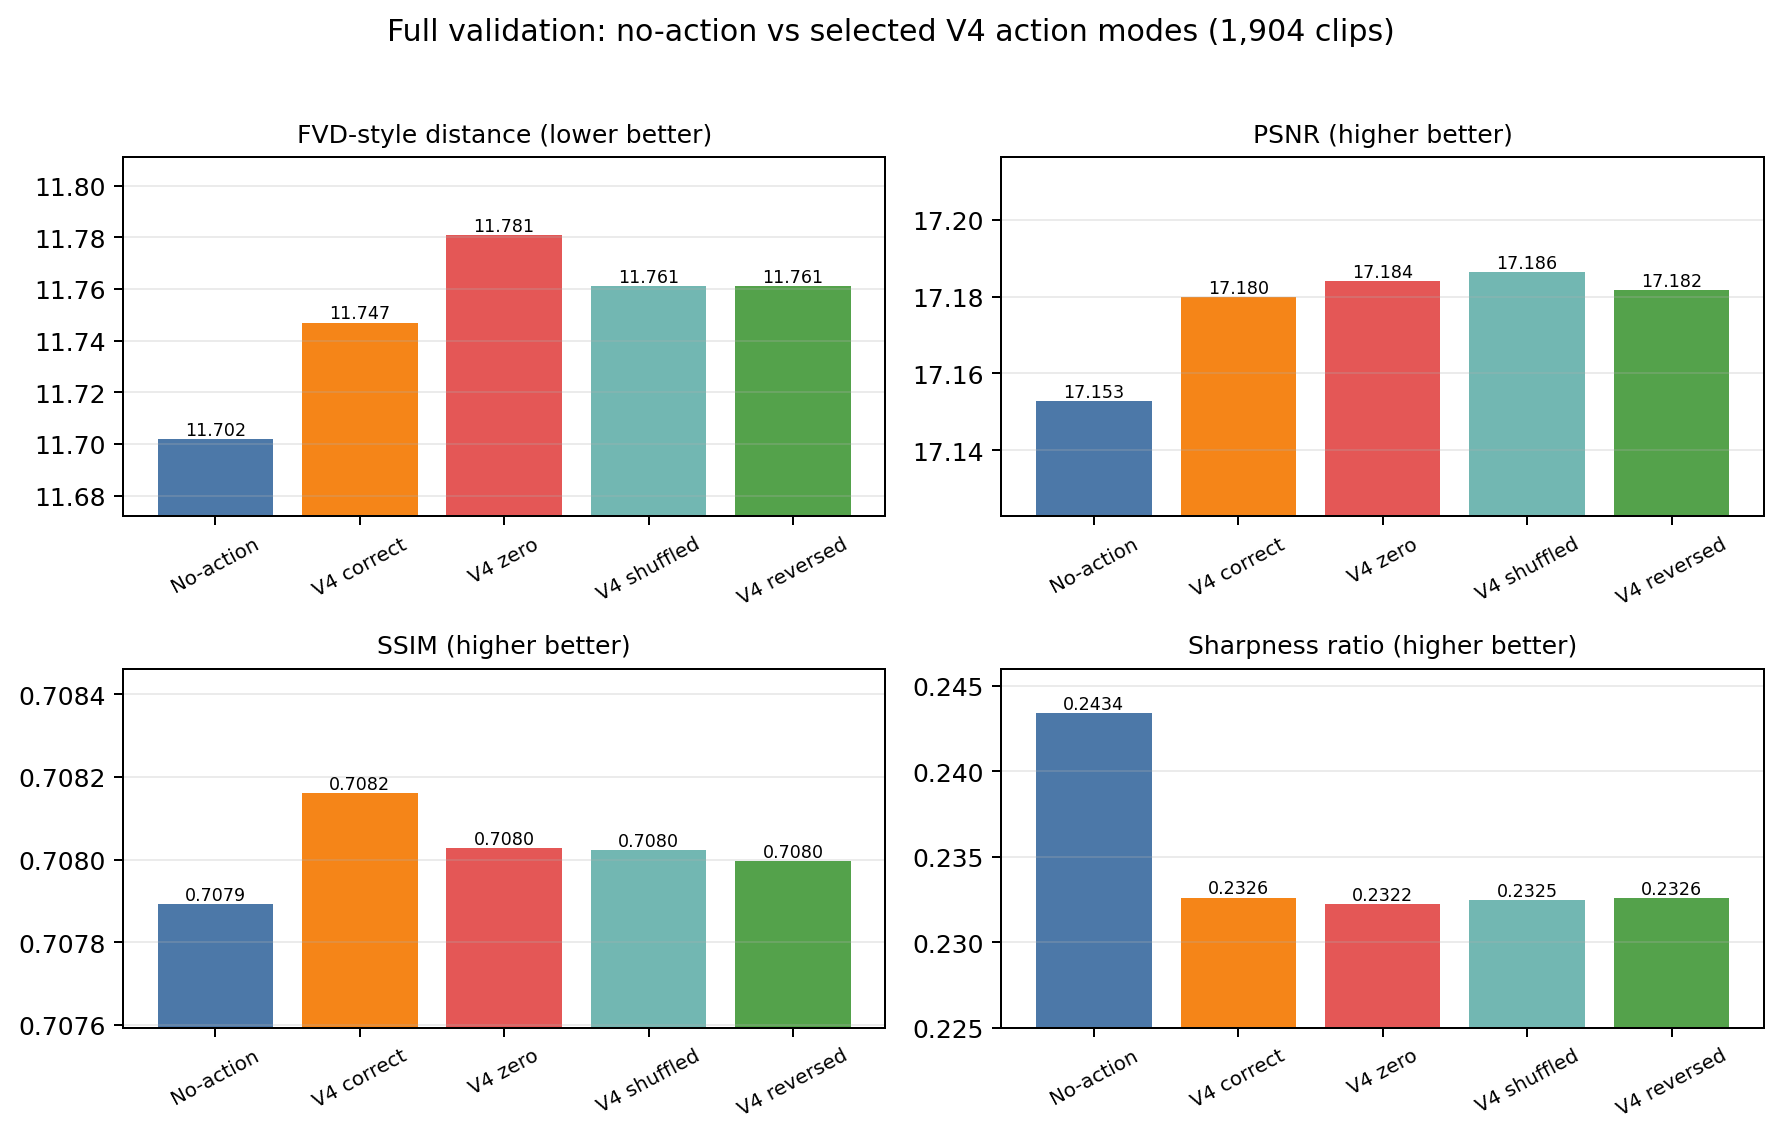
\includegraphics[width=0.95\linewidth]{figures/fullval_model_mode_quality.png}
\caption{Full validation across no-action and V4 action modes. The selected action model is compared not only to no-action, but also to wrong-action generations. Correct actions are the best V4 mode by FVD-style distance while remaining visually close to no-action.}
\label{fig:fullval}
\end{figure*}

\subsection{Correct actions versus wrong actions}

Action sensitivity alone could mean the model changes arbitrarily when actions change. We therefore stratify validation windows by action magnitude. The high-action stratum is the union of braking, acceleration, and turning windows. Table~\ref{tab:strata} shows the strongest semantic result: on high-action clips, correct actions are slightly closer to the recorded future than wrong actions.

\begin{table}[t]
\centering
\caption{Correct-vs-wrong advantage by stratum. Positive $\Delta$PSNR/$\Delta$SSIM means correct actions are closer to ground truth than wrong actions.}
\small
\begin{tabular}{lrrrr}
\toprule
\textbf{Stratum} & \textbf{clips} & $\mathbf{\srgb}$ & $\Delta$PSNR & $\Delta$SSIM\\
\midrule
All & 1904 & 2.262 & -0.00419 & +0.00015\\
High action & 1055 & 2.303 & +0.00192 & +0.00027\\
Accelerate & 408 & 2.484 & +0.00493 & +0.00069\\
Turning & 509 & \textbf{2.547} & +0.00419 & +0.00054\\
Brake & 402 & 2.041 & -0.00064 & -0.00003\\
Low action & 571 & 2.335 & -0.01786 & -0.00001\\
\bottomrule
\end{tabular}
\label{tab:strata}
\end{table}

The effect is small, but the sign is important. It is strongest on acceleration and turning, where future ego actions should be most informative. Braking remains weak, and low-action clips are not the right controllability test because the future is already strongly determined by visual context.

\begin{figure*}[t]
\centering
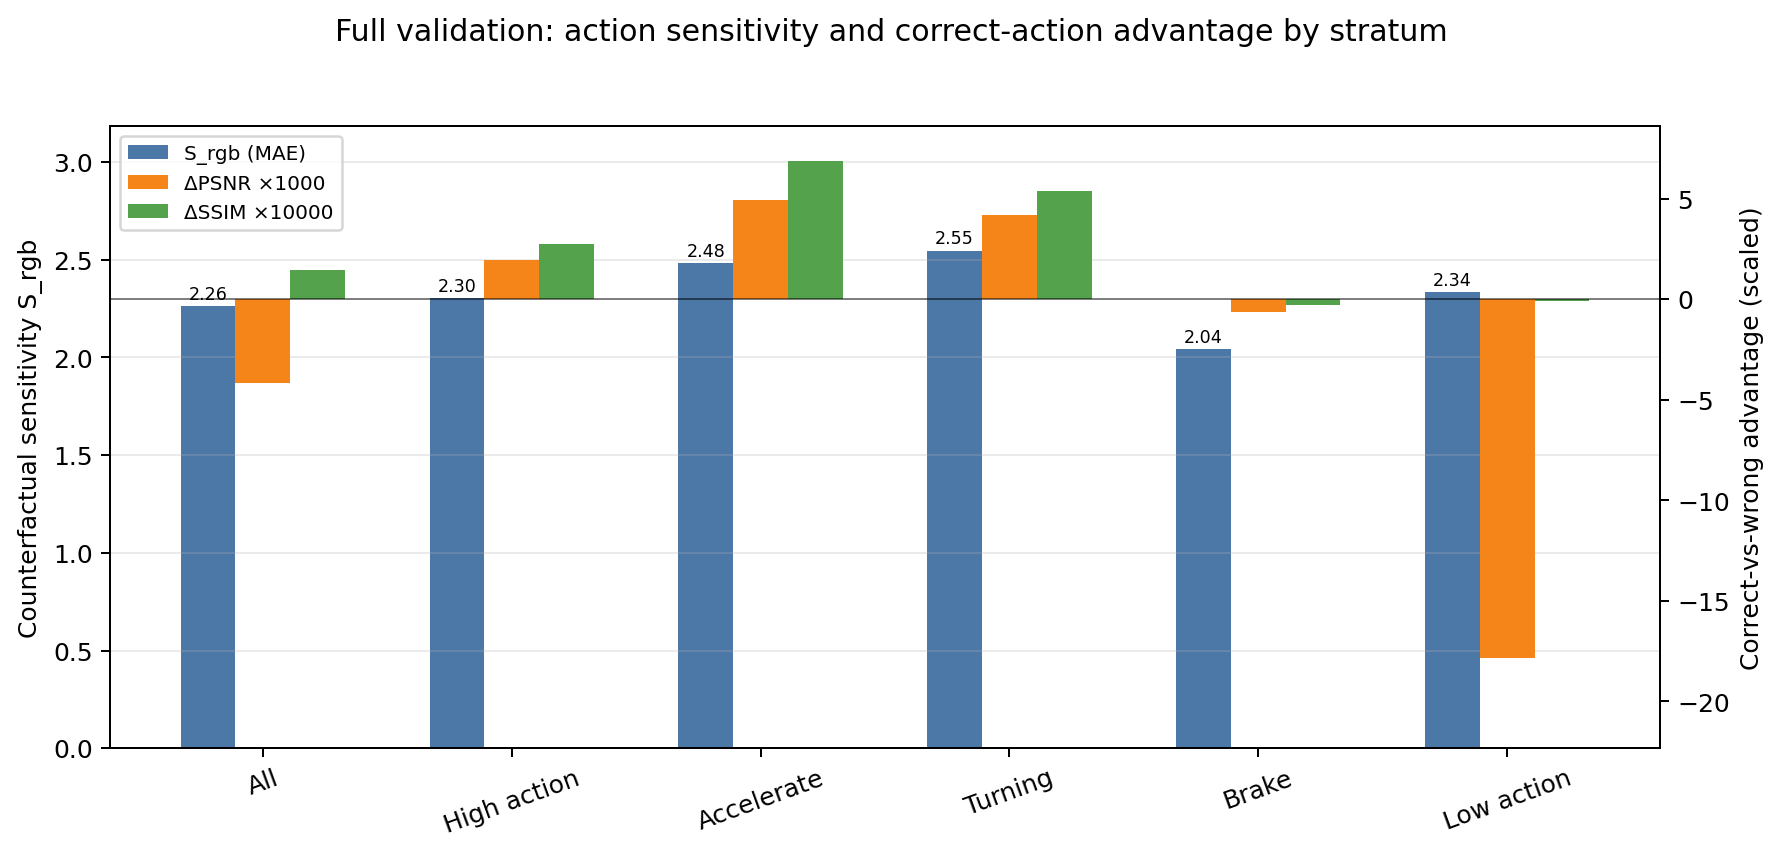
\includegraphics[width=0.95\linewidth]{figures/stratum_action_alignment.png}
\caption{Action sensitivity and correct-action advantage by stratum. The model is most sensitive on turning and acceleration clips, and those same strata show positive correct-vs-wrong PSNR/SSIM advantage.}
\label{fig:strata}
\end{figure*}

\subsection{Why naive action conditioning was insufficient}

Table~\ref{tab:diagnostic} and Fig.~\ref{fig:diagnostic} summarize the core diagnostic that changed the project direction. AdaLN-style action conditioning achieved the best PSNR and SSIM on the 512-window diagnostic subset, but it did so by collapsing sharpness and motion. This is exactly the failure mode we wanted to avoid.

\begin{table}[t]
\centering
\caption{512-window diagnostic subset. AdaLN improves PSNR/SSIM but collapses sharpness and motion.}
\small
\begin{tabular}{lrrrr}
\toprule
\textbf{Model} & \textbf{PSNR} & \textbf{SSIM} & \textbf{Sharp.} & \textbf{Motion}\\
\midrule
No-action & 16.893 & 0.695 & 0.250 & \textbf{1.262}\\
Frame AdaLN & \textbf{19.539} & \textbf{0.795} & 0.120 & 0.511\\
HF-teacher v2 & 17.970 & 0.731 & 0.140 & 0.927\\
V4 action-strong & 17.803 & 0.724 & 0.164 & 0.995\\
V4 main text & 16.844 & 0.691 & 0.245 & 1.216\\
\bottomrule
\end{tabular}
\label{tab:diagnostic}
\end{table}

\begin{figure}[t]
\centering
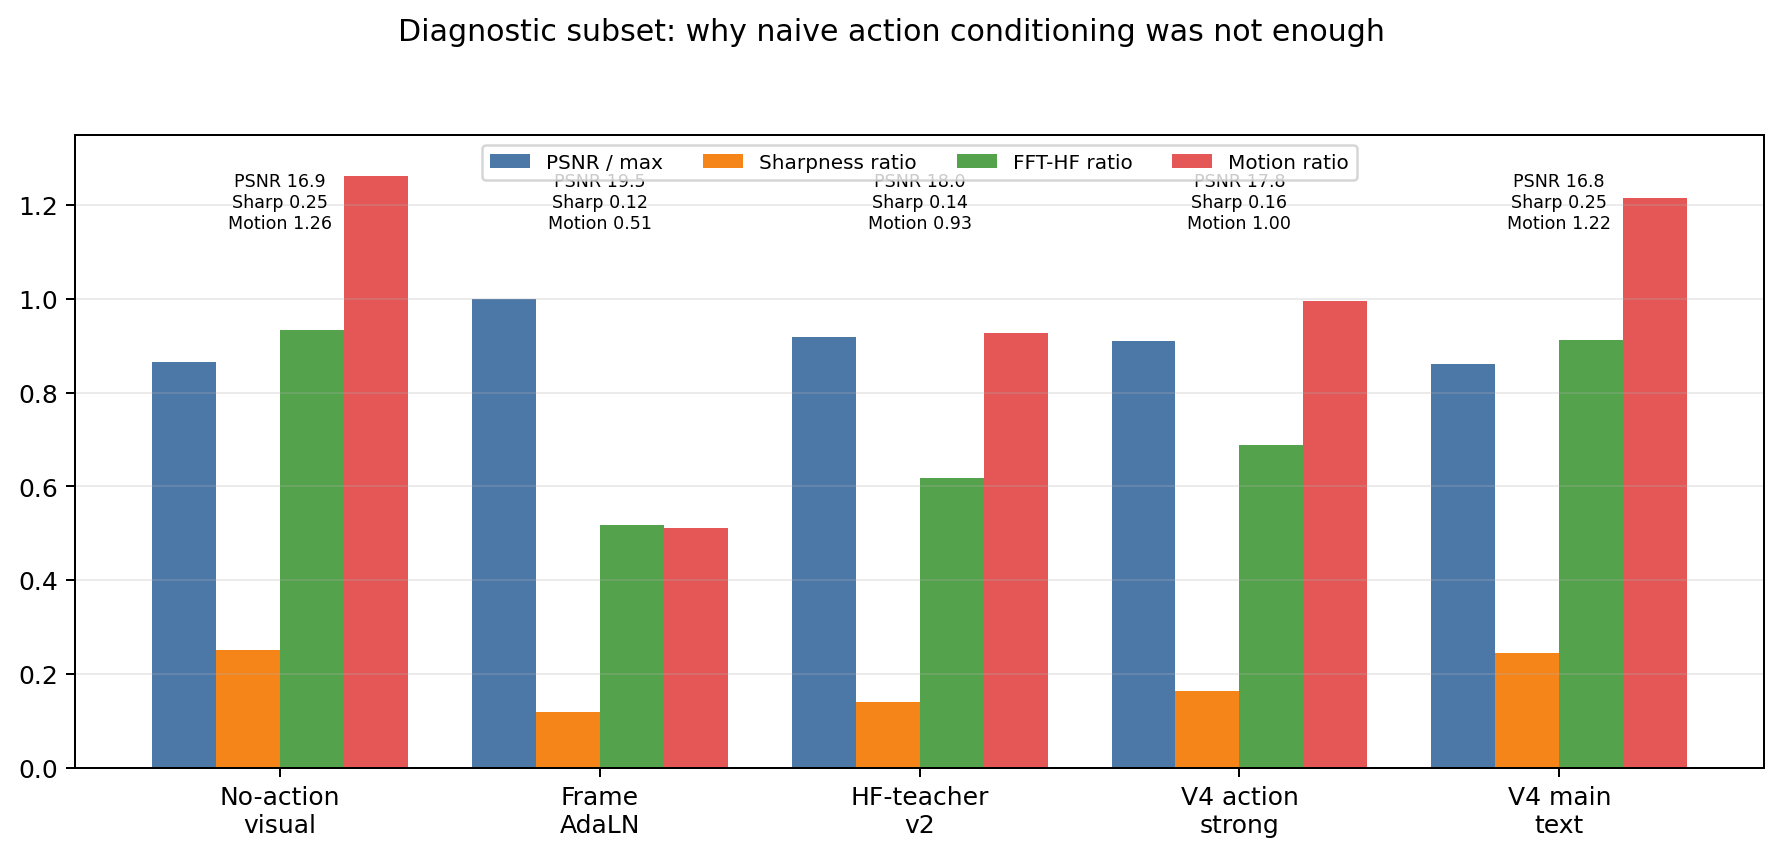
\includegraphics[width=\linewidth]{figures/method_evolution_quality_tradeoff.png}
\caption{Diagnostic subset comparison. The high-PSNR AdaLN model loses high-frequency detail and motion. The final V4 direction preserves these quantities closer to the no-action visual model.}
\label{fig:diagnostic}
\end{figure}

\subsection{Capacity and checkpoint behavior}

We also tested whether dense 112D action conditioning was limited by adaptation capacity. Rank 32 briefly reached higher sensitivity, but was unstable. Rank 64 gave the selected tradeoff. Rank 128 was not a monotonic improvement.

\begin{table}[t]
\centering
\caption{Capacity sweep on 5-clip checkpoint diagnostics. Rank 64 was selected because it offered high sensitivity with better stability than rank 32 and no clear degradation like rank 128.}
\small
\begin{tabular}{lrrrr}
\toprule
\textbf{Model} & \textbf{Step} & $\mathbf{S}$ & \textbf{FVD} & \textbf{PSNR}\\
\midrule
Rank 32 & 10,000 & \textbf{3.893} & 88.303 & 17.257\\
Rank 32 & 23,976 & 1.904 & 89.231 & 17.257\\
Rank 64 & 10,000 & 2.454 & \textbf{82.769} & 17.278\\
Rank 64 & 18,000 & 3.499 & 86.108 & \textbf{17.298}\\
Rank 64 & 23,976 & 3.157 & 86.805 & 17.269\\
Rank 128 & 15,000 & 2.591 & 85.809 & 17.276\\
\bottomrule
\end{tabular}
\label{tab:capacity}
\end{table}

\begin{figure}[t]
\centering
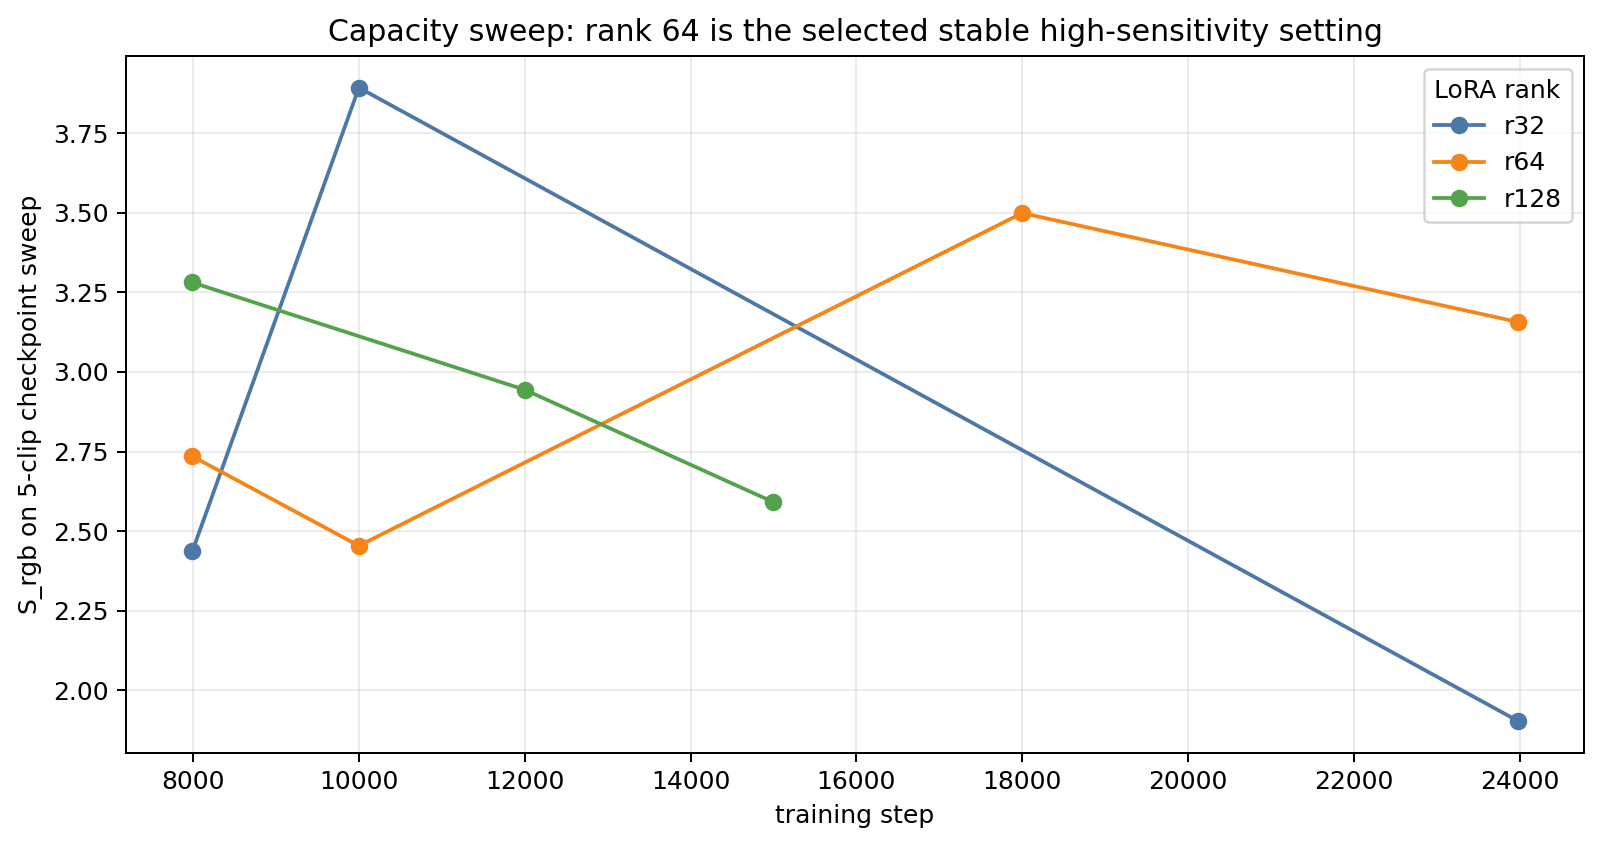
\includegraphics[width=\linewidth]{figures/capacity_sensitivity_over_checkpoints.png}
\caption{Action sensitivity over checkpoints for rank 32, 64, and 128. Higher rank is not automatically better; the final selected checkpoint is a stability/quality/sensitivity tradeoff.}
\label{fig:capacity}
\end{figure}

\section{Discussion}

\textbf{What improved?}
The cleanest improvement is controllability. The no-action model has $\srgb=0.000$ by construction. The final model reaches $\srgb=2.262$ on full validation and $\srgb=2.303$ on high-action clips. It does this while staying visually close to no-action: FVD changes from 11.702 to 11.747, PSNR from 17.153 to 17.180, and SSIM from 0.70789 to 0.70816.

\textbf{Why is the result not just noise?}
The final validation includes 1,904 windows and compares correct actions against three wrong-action modes. Correct actions are not globally better on every window, but they become positive on the high-action subset and especially on acceleration and turning. This is the expected direction if actions matter primarily when the future is not determined by context alone.

\textbf{What remains unsolved?}
The correct-vs-wrong advantage is small. Braking is not solved. The action-conditioned model is not visually superior to no-action on every metric. The result should be framed as a transition from action-blind prediction to measurable action sensitivity and early semantic alignment, not as a complete driving simulator.

\textbf{Why this is still a useful finding.}
The project tested many plausible action-conditioning mechanisms and found a consistent pattern: uncontrolled action injection damages visual synthesis, while low-frequency temporal conditioning plus high-frequency preservation produces the best tradeoff. This is aligned with recent work emphasizing temporal consistency, feature alignment, and multi-condition structure in video diffusion~\cite{luo2025enhanceavideo,lee2025align4gen,yi2025conditionalcompression}.

\section{Conclusion}

We studied action conditioning for pretrained diffusion-transformer driving video generation. The main finding is that action control and visual fidelity are separate axes. A no-action model gives strong visual prediction but zero controllability. Naive action conditioning can increase pixel metrics while destroying sharpness and motion. Our final low-frequency action-conditioned model improves counterfactual sensitivity from $\srgb=0.000$ to $\srgb=2.262$ on full validation while preserving near-baseline PSNR, SSIM, and FVD-style distance. On high-action clips, correct actions are slightly closer to ground truth than wrong actions. The result is not a solved world model, but it is a clear and defensible step toward controllable driving video generation.

{\small
\bibliographystyle{ieee}
\bibliography{references}
}

\end{document}
